\documentclass[border=10pt]{standalone}
\usepackage{tikz}
\usetikzlibrary{
  calc
}
\usepackage{pgfplots}

% https://tex.stackexchange.com/questions/218569/define-stretchable-shading
\newbox\shbox
\tikzset{
  path picture shading/.style={
    path picture={
        \pgfpointdiff{\pgfpointanchor{path picture bounding box}{south west}}
        {\pgfpointanchor{path picture bounding box}{north east}}
        \pgfgetlastxy\pathwidth\pathheight
        \pgfinterruptpicture
        \global\setbox\shbox=\hbox{\pgfuseshading{#1}}
        \endpgfinterruptpicture
        \pgftransformshift{\pgfpointanchor{path picture bounding box}{center}}
        \pgftransformxscale{\pathwidth/(\wd\shbox)}
        \pgftransformyscale{\pathheight/(\ht\shbox)}% \dp will (should) be 0pt
        \pgftext{\box\shbox}
    }
  }
}
\pgfdeclarehorizontalshading{spectrum}{50bp}{
    color(0.00000000000000bp)=(violet);
    color(8.33333333333333bp)=(blue);
    color(16.66666666666670bp)=(cyan);
    color(25.00000000000000bp)=(green);
    color(33.33333333333330bp)=(yellow);
    color(41.66666666666670bp)=(orange);
    color(50.00000000000000bp)=(red)
}
% \definecolor{myleftcolor}{rgb}{0.5020, 0, 0}
% \definecolor{myrightcolor}{rgb}{0, 0, 0.7059}

\pgfplotsset{
  colormap={spectrum}{
    color(0.00000000000000bp)=(violet);
    color(8.33333333333333bp)=(blue);
    color(16.66666666666670bp)=(cyan);
    color(25.00000000000000bp)=(green);
    color(33.33333333333330bp)=(yellow);
    color(41.66666666666670bp)=(orange);
    color(50.00000000000000bp)=(red)
  }
}
\begin{document}


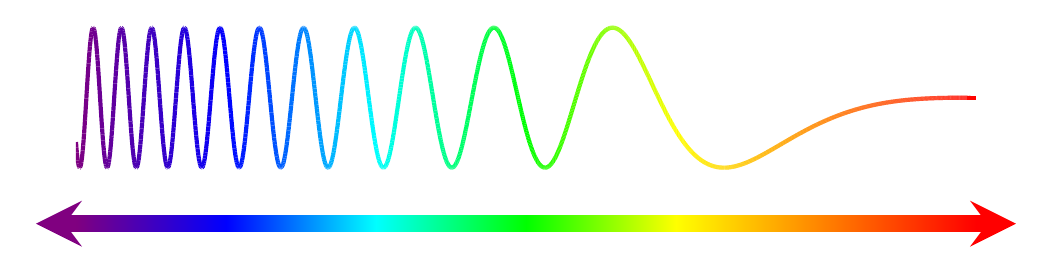
\begin{tikzpicture}
  % define the unit
  [x=1in, y=0.35in]
  \shade[
    path picture shading=spectrum
  ] (0, -3pt) rectangle (4.5, 3pt);
  \draw[
    ->, >=stealth,
    line width=6pt, anchor=east, color=violet
  ] (0, 0) -- ++(-0.2, 0);
  \draw[
  ->, >=stealth,
  line width=6pt, anchor=west, color=red
  ] (4.5, 0) -- ++(0.2, 0);

  \begin{axis}
    [
      % tell pgfplot to use the same unit as tikz
      x=1in, y=0.35in,
      % the size of pgfplot
      % width=5in, height=1in,
      % set the domain of the function
      domain=-4.5:0,
      % only show the domain
      xmin=-4.5, xmax=0,
      ymin=-1.8,
      % do not show the spines of the axes
      axis lines=none,
      % define the colormap, bluered inverted
      colormap name=spectrum,
      % colormap={reverse bluered}{
      %   indices of colormap={
      %       \pgfplotscolormaplastindexof{bluered},...,0 of bluered}
      % },
    ]
    \addplot[
      mesh, point meta=x,
      % number of points
      samples=2000,
      line width=1.5pt,
    ] {
      % the function of the spectrum
      sin(45*x^3)
    };
  \end{axis}
\end{tikzpicture}

\end{document}
